\documentclass[]{article}
\usepackage[margin = 1.3in]{geometry}

%opening
\title{Quantum Random Number Generation from Shot Noise and Phase-induced Intensity Noise}
\author{Robin Camphausen}
\date{}
%\usepackage[sorting=none]{biblatex}
%\bibliography{bibliographyFibreEye}
\usepackage{graphicx}
\usepackage{float}
\usepackage[font = {small,it}]{caption}
%\usepackage{subcaption}
\usepackage{cite}
%\bibliographystyle{unsrt}
%\usepackage{notoccite}
\usepackage{gensymb}
\usepackage{textcomp}
\usepackage{amsmath}
\usepackage{hyperref}
\usepackage[
    % font={small,sf},
    % labelfont=bf,
    % format=hang,    
    % format=plain,
    margin=0pt,
    width=0.8\textwidth,
]{caption}
\usepackage[list=true]{subcaption}
\usepackage{graphicx} %Loading the package
\graphicspath{{../../Pictures/SPAD-QRNG/}}


\newcommand*\mean[1]{\overline{#1}}


\begin{document}
\maketitle
\section{Introduction}

	Quantum random number generators (QRNGs) are important for a large number of applications, including for finance, communication and computational modelling \cite{herrero-collantes_quantum_2017}. One way to generate quantum random numbers (QRNs) is to measure shot noise, which arises due to the quantised nature of light: when observing a light source over a given time frame a discrete number of photons will arrive at the detector and while the average number of photons stays constant there is a variance in the number of arrivals per time frame \cite{sanguinetti_quantum_2014}. It is also possible to generate QRNs by measuring phase noise, which is due to the fact that a spontaneously emitted photon has a completely random phase, uniformly distributed between $0$ and $2\pi$ \cite{xu_ultrafast_2012,abellan_ultra-fast_2014}. In this report we describe a hybrid QRNG method, which increases the randomness able to be extracted in the Shot noise method by also taking into account the random optical phases of the light source.

\section{Phase-induced Intensity Noise} \label{RPS}

	A single spontaneously emitted photon has random phase, but it is of course not possible to measure the phase of a single photon. In references \cite{abellan_ultra-fast_2014,mitchell_strong_2015,abellan_generation_2015} therefore, the single spontaneously emitted photon is generated inside a laser cavity, which subsequently uses stimulated emission to generate many copies of this first photon until the light intensity is large enough for an interferometric measurement of the phase. The laser must subsequently be switched off again to allow all stimulated photons in the cavity to decay, so that upon switching it on again a new spontaneously emitted photon with a new random phase can start the same process again.
	Another way of exploiting the random phase of a spontaneously emitted photon is to measure many of them at once. If all the photons are emitted such that they have statistically independent amplitudes and phases from each other, the resulting sum can be described as a Random Phasor Sum (RPS) \cite{goodman_statistical_2000}:
		\begin{equation}
		\mathbf{a} = ae^{i\theta} = \frac{1}{\sqrt{N}} \sum_{k=1}^{N} \alpha_k e^{i\phi_k}. \label{eq:RPSbasic} 
		\end{equation}
	Note that this equation is normalised. $\alpha_k /\sqrt{N}$ and $\phi_k$ are the amplitudes and phases respectively of the $K^{th}$ photon comprising the RPS. In general $\alpha_k$ can take on any distribution with some mean $\mean{\alpha}$ and second moment $\mean{\alpha^2}$. We let $\phi_k$ be uniformly distributed over $[0,2\pi)$. As $N$ gets very large, by the central limit theorem $\mathbf{a}$ becomes a Gaussian random variable. In particular, following Chapter 2.9 from \cite{goodman_statistical_2000}, the joint density function of the real(imaginary) components $re$($im$) of $\mathbf{a}$ is
		\begin{equation}
		P_{a}(re,im) = \frac{1}{2\pi \sigma^2} e^{-\frac{re^2+im^2}{2 \sigma ^2}},
		\end{equation}
	where $\sigma^2 = \mean{\alpha^2}/2$. Converting this back to the polar coordinates $a$ and $\theta$ we obtain
		\begin{equation}\label{eq:normRPSpolar}
			P_a(a,\theta)= 
		\begin{cases}
		    \frac{a}{2\pi \sigma^2} e^{-\frac{a^2}{2 \sigma ^2}},& \text{if } 0 \leq \theta < 2\pi,\> a>0,\\
		    0,              & \text{otherwise.}
        \end{cases}
        \end{equation}
    Note that this equation is still uniformly distributed for $\theta$. Now for the case of summing up photons, equation \ref{eq:normRPSpolar} describes the distribution of amplitude $a$ and phase $\theta$ of a normalised electric field. At a given moment in time $\tau$ the instantaneous amplitude(phase) is $a_\tau$($\theta_\tau$), where the mean and variance respectively of $a$ are $\mean{a} = \sqrt{\pi/2}\sigma$ and $\sigma_a^2 = (2-\pi/2)\sigma^2$.

    However, when detecting light we actually measure the intensity $I = |\mathbf{a}|^2$. To find the distribution as well as the mean and standard deviation of the instantaneous intensity $I_\tau$ we make the substitution $I_\tau = a_\tau ^2$ and use the relation $P_I(I)=P_A(A=\sqrt{I})\>|dA/dI|$, as well as the statistical properties of the mean and variance (Chapter 4.2 \cite{goodman_statistical_2000}):
    	\begin{eqnarray}
    		P_I(I)&=&
		\begin{cases}
			\frac{1}{2\sigma^2} e^{-\frac{I}{2 \sigma ^2}},& \text{if } I \geq 0,\\
		    0,              & \text{otherwise,}
		\end{cases}
		\\
			\sigma_I &=& \mean{I} = 2\sigma^2 = \mean{\alpha^2}. \label{eq:RPSstats}
		\end{eqnarray}
	That is to say, even if the amplitude $\alpha$ of the photons being summed has no variation at all (as long as $\alpha$ is non-zero), the resulting instantaneous intensity of the RPS randomly varies with a standard deviation equal to the mean of the intensity ($\sigma_I = \mean{I}$). This variation is therefore known as phase-induced intensity noise (PIIN). Note that this PIIN superficially appears similar to photon shot noise (in particular eq. \ref{eq:RPSstats}), however there is an important difference: in equation \ref{eq:RPSbasic} we summed $N$ phasors each with amplitude $\alpha_k /\sqrt{N}$. While we denoted this as the amplitude of individual photons, there is no reason why each individual phasor cannot be composed of many photons: This would be the case if summing many independent laser modes (out of phase with each other) which each individually contain many in-phase photons. In this case the variance due to PIIN would remain the same, whereas the shot noise would be much smaller due to the large number of photons.

\section{Measuring PIIN}
	
	The RPS from section \ref{RPS} in fact accurately describes the majority of light sources available today: incandescent light bulbs, light emitting diodes (LEDs) and amplified spontaneous emission (ASE) all generate light from spontaneously emitted photons; this is also known as thermal light. Moreover, it has already been shown that it is possible to measure PIIN and subsequently extract random numbers from it. This was done by directly measuring the intensity fluctuations of an ASE source \cite{argyris_sub-tb/s_2012}, interfering an ASE source with itself \cite{li_random_2014} and by measuring the intensty fluctuations of a superluminescent LED (SLED - essentially a semiconductor laser diode without a cavity) \cite{huang_real-time_2014, li_scalable_2011}.\\
	Now, equation \ref{eq:RPSstats} refers to the fluctuations in the \textit{instantaneous} intensity produced by a thermal light source. However, any real device that measures light has a finite bandwidth, and therefore integrates the measured intensity over a non-zero period of time. To see how this affects the measurement we start with an intuitive first-order approximation of thermal light as follows: We model a single mode of incoherent light as an ideal monochromatic sine wave, interrupted by random phase shifts every period $\tau_c$, where $\tau_c$ is the coherence time (see fig. \ref{fig:simpleThermal_oneMode}).
		\begin{figure}[h]
		\centering
		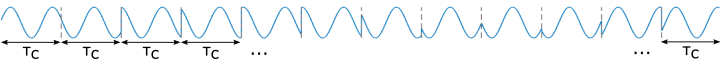
\includegraphics[width=0.9\textwidth]{simpleThermal_oneMode.png}
		\caption{\label{fig:simpleThermal_oneMode} Simple model of a single mode of thermal light: Modelled as a perfect sinusoidal wave interrupted by random phase jumps every coherence time $\tau_c$.}
		\end{figure}
	When two of these thermal modes are added together (this could represent a spontaneous emission source generating two photons at a time, or a laser with two independent modes) the waves interfere causing a different combined intensity for each $\tau_c$ period depending on the phase difference between the two modes (see fig. \ref{fig:simpleThermal_twoModes}).\\
		\begin{figure}[h]
		\centering
		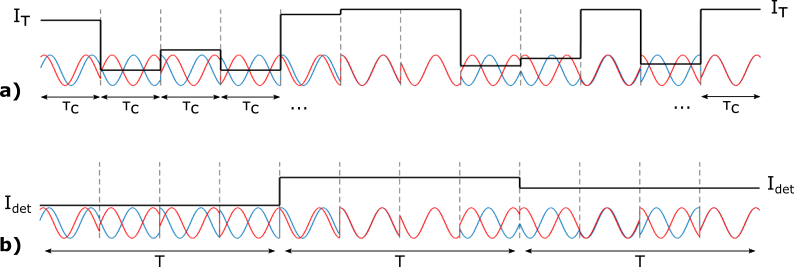
\includegraphics[width=1\textwidth]{simpleThermal_twoModes.png}
		\caption{\label{fig:simpleThermal_twoModes} Simple model of the origin and detection of PIIN: when two (or more) modes of thermal light interfere with each other, the random phase jumps will cause a random phase difference between the modes for each period $\tau_c$. \bf{a)} \normalfont The instantaneous intensity $I_{\tau}$ fluctuates strongly from one coherence period $\tau_c$ to the next, due to the modes interfering constructively or destructively depending on the instantaneous phase difference. \bf b) \normalfont When detecting for an integration time $T$ longer than the coherence time (in this case $T=4\tau_c$) the fluctuations in detected intensity $I_{det}$ weaker, as the integration averages out large fluctuations over multiple coherence times.}
		\end{figure}
	The normalised measured instantaneous intensity for each period $\tau$, given some phase difference between the two modes $\Delta \phi$, is $I_{\tau} = \frac{1+cos(\Delta \phi)}{2}$. Note that $\Delta \phi_k$ is uniformly distributed over $[0,2\pi)$. However, if the integration time of the detector $T$ is larger than the coherence time $\tau_c$ we can define the ratio $M$ as follows:
		\begin{equation}
		M = T/\tau_c.
		\end{equation}
	The normalised detected intensity thus becomes
		\begin{equation}
		I_{det} = \sum_{m=1}^M \frac{1}{M} \frac{1+cos(\Delta \phi_m)}{2}.
		\end{equation}
	Using the statistical properties of the cosine function, and the central limit theorem, we thus obtain the mean and standard deviation of the \textit{measured} intensity:
		\begin{equation}
		\mean{I}_{det} = \frac{1}{2}, \quad \sigma_{det} = \frac{1}{\sqrt{8M}} \label{eq:simpleTwoMode_stats}.
		\end{equation}
	Importantly, what eq. \ref{eq:simpleTwoMode_stats} shows is that as the integration time $T$ gets much larger than the coherence time $\tau_c$, the ratio $M$ becomes large and the standard deviation in the detected intensity fluctuation tends to zero. This simple model therefore yields three important conclusions: Firstly, eq. \ref{eq:simpleTwoMode_stats} is consistent with our everyday experience, because for thermal light sources commonly encountered (such as incandescent lightbulbs) the coherence time is much shorter than the integration time of the human eye - and thus the PIIN is not readily observed. Secondly it indicates that to extract random numbers from PIIN the light must be measured fast, and indeed the faster it is measured the more randomness can be extracted. And thirdly, as measured noise is proportional to $1/\sqrt{M} = \sqrt{\tau_c}/\sqrt{T}$, increasing the coherence time of the thermal light source will also increase the measured noise.
	
	Even though we derived  eq. \ref{eq:simpleTwoMode_stats} for a very simple two-mode light model, the statistical properties of a fully incoherent light source are very similar (see chapter 6 in \cite{goodman_statistical_2000}). In particular, in the limit where $T>>\tau_c$, i.e. of a much longer integration time than coherence time, the measured PIIN is described by
		\begin{equation} 
		\frac{\sigma_{det}}{\mean{I}_{det}} = \frac{1}{\sqrt{M}} = \sqrt{\frac{\tau_c}{T}}.
		\label{eq:fullPIINstats}
		\end{equation}
	The coherence time $\tau_c$ can be approximated in terms of the light source's centre wavelength $\lambda$ and spectral width $\Delta\lambda$ as follows:
		\begin{equation}
		\tau_c = \frac{\lambda^2}{c\Delta\lambda},
		\label{eq:coherenceTime}
		\end{equation}
	where $c$ is the speed of light. By substituting $lambda$ and $\Delta\lambda$ values for typical incoherent light sources such as LEDs or SLEDs into eq. \ref{eq:coherenceTime} we can see that $\tau_c$ is on the sub-picosecond timescale. Integration times of photodetectors on the other hand are normally at least two orders of magnitude larger and thus we can apply \ref{eq:fullPIINstats} as we are comfortably in the $T>>\tau_c$ regime.

\bibliographystyle{ieeetr}
\bibliography{cameraQRNG_bib}

\end{document}